\section{SIFT}
SIFT (Scale Invariant Feature Transform) was  proposed by David Lowe, and published in the original paper \cite{Lowe1999} in 1999. SIFT.

Compared to ordinary techniques such as the Harris Corner Detector \cite{Harris1988} or Canny edge detector \cite{Canny1986}, the SIFT identifies the general (not only edges and corners) key-points. The descriptors, which describe the local image region around the key-points are scale invariant. Moreover, they are invariant to rotation, illumination and to change in affine transformations. In our text, we introduce the methodology of training the classifier that recognizes the objects in real images (photographs); therefore the properties of SIFT feature vector are essential.

\subsection{Key-point Detection}

Let us consider an input image \( I_{img}(x,y) \). A convolution of the image with a Gaussian kernel
\begin{equation}
    G(x,y,\sigma) = \frac{1}{2\pi\sigma^2}e^{-\frac{x^2+y^2}{2\sigma^2}},
    \label{eq:Gaussian_kernel}
\end{equation}
at a scale \( \sigma \) is exploited to get a scale-space representation of the image, so that:
\begin{equation}
    L(x, y,\sigma) =  G(x,y,\sigma)*I_{img}(x,y).
\end{equation}

In order to detect scale invariant key-points, scale normalised Laplacian of Gaussian (LoG)
\begin{equation}
    \Laplace_{norm} L(x, y, \sigma) = \sigma\left(\frac{\partial^2 L(x,y,\sigma)}{\partial x^2} + \frac{\partial^2 L(x,y,\sigma)}{\partial y^2}\right)
\end{equation}
is required \cite{Koenderink1984}. It has been shown \cite{Mikolajczyk2002}, that local extrema of LoG provide the most stable image features, compared to many other popular image functions.

Determination of the LoG would be time consuming, therefore, it is approximated by the Difference of Gaussian (DoG)\cite{Lowe2004}.The DoG is computed from two adjacent scales separated by a constant multiplicative factor $k \in \mathbb{R}$:
\begin{equation}
    D(x,y,\sigma) := L(x,y,k\sigma) - L(x,y,\sigma).
\end{equation}

To ensure scale invariance, the extrema are located not only in the domain of one DoG, however it is found across different scales as well. The different DoGs at the scales are created by progressively convolving the original image with the Gaussian kernel. The consecutive Gaussian kernels' scale differs by the multiplicative factor $k$.

At each doubling of the scale $k$, the resolution of an image can be reduced by factor of $2$ for efficiency. Each group of blurred images of the same resolution is called an octave. In each octave, we generate the DoG by subtracting the $L(x, y, \sigma)$ of neighbouring scales. This is called the DoG pyramid and can be seen in \figref{fig:DoG_pyramid}.

\begin{figure}
    \centering
    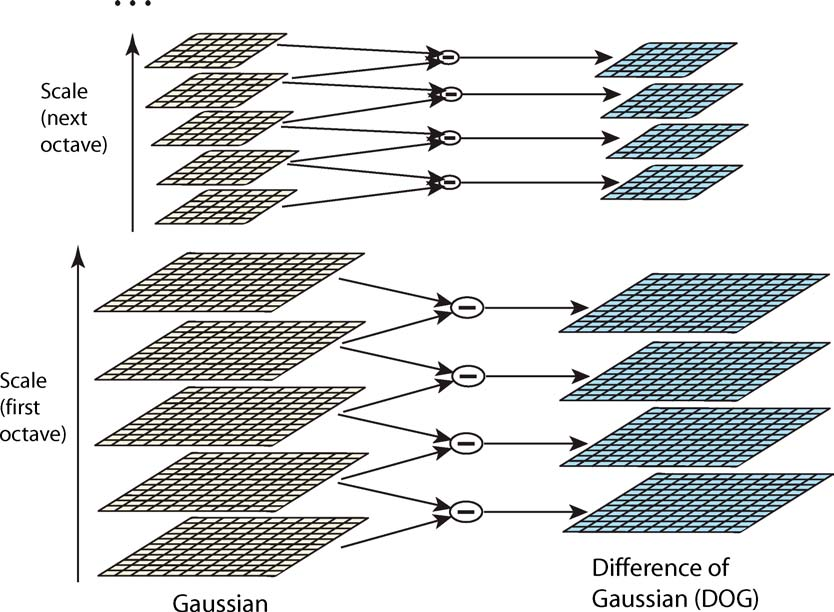
\includegraphics[width=0.8\textwidth]{Figures/sift/pyramid.jpg}
    \caption[DoG pyramid.]{DoG pyramid. \cite{Lowe2004}}
    \label{fig:DoG_pyramid}
\end{figure}

Each pixel in the DoG pyramid is compared to the $3\times3$ pixels in DoGs below and above, and to the $8$ surrounding pixels. This is shown in \figref{fig:DoG_extrema}. The pixel is selected as a key-point candidate, if it has lower or higher value than all of these $26$ pixels.

\begin{figure}
    \centering
    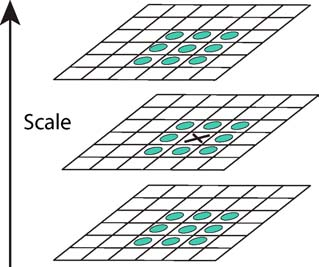
\includegraphics[width=0.4\textwidth]{Figures/sift/extrema.jpg}
    \caption[Optima of the DoG are selected by the means of comparing pixel to the 26 pixels surrounding it in the scale-space.]{Optima of the DoG are selected by the means of comparing pixel to the 26 pixels surrounding it in the scale-space. \cite{Lowe2004}}
    \label{fig:DoG_extrema}
\end{figure}

To detect a sub-pixel locations of extrema, the DoG is interpolated using quadratic Taylor expansion at each key-point candidate:
\begin{equation}
    D(\boldsymbol{x}) = D + \frac{\partial D^T}{\partial \boldsymbol{x}}\boldsymbol{x}+\frac{1}{2}\boldsymbol{x}^T\frac{\partial^2 D}{\partial \boldsymbol{x}^2}\boldsymbol{x},
    \label{eq:taylor_expansion}
\end{equation}
where \( D(x,y,\sigma) \) and the partial derivatives are evaluated at the key-point and \( \boldsymbol{x}=(x,y,\sigma) \) is the offset from the key-point. Then, extrema \( \hat{\boldsymbol{x}} \) is located by setting the gradient of \( D \) to be zero vector:
\begin{equation}
    \hat{\boldsymbol{x}} = - \frac{\partial^2 D^{-1}}{\partial \boldsymbol{x}^2}\frac{\partial D}{\partial \boldsymbol{x}}.
    \label{eq:taylor_extremum}
\end{equation}
If the offset \( \hat{\boldsymbol{x}} \) is larger than \( 0.5 \) in any dimension, it indicates that the extrema is closer to another point. In this case, the candidate point is changed to the new point and interpolation is performed again.

The function value at the sub-pixel extrema ,$D(\hat{\boldsymbol{x}})$, is used for rejecting extrema with low contrast. In our experiments, we use the OpenCV SIFT implementation default value $\frac{0.04}{3}$\cite{openCV}.

The DoG has a strong response along edges, even if the location along the edge is poorly determined. These candidate key-points have principal curvature perpendicular to the edge much larger than the principal curvature along it. The principal curvatures can be computed from a $2\times2$ Hessian matrix at the location of the key-point candidate
\begin{equation}
    \boldsymbol{H} =
    \begin{bmatrix}
        D_{xx} & D_{xy}\\
        D_{xy} & D_{yy}
    \end{bmatrix},
    \label{eq:hessian}
\end{equation}
where the partial derivatives are estimated by taking the differences of neighboring sample points. The eigenvalues of $\boldsymbol{H}$ are proportional to the principal curvatures.

The computation of eigenvalues can be avoided, as only the ratio of the eigenvalues is required. Let us denote the larger eigenvalue as $\alpha$ and the smaller one as $\beta$. The trace of $\boldsymbol{H}$ is defined as
\begin{equation}
    Tr(\boldsymbol{H}) = D_{xx}+D_{yy} = \alpha+\beta,
\end{equation}
and the determinant as
\begin{equation}
    Det(\boldsymbol{H}) = D_{xx}D_{yy}-D_{xy}^2 = \alpha\beta.
\end{equation}

Let $r$ be the ratio of the eigenvalues, such that
\begin{equation}
    r=\frac{\alpha}{\beta}.
\end{equation}
Then,
\begin{equation}
    \frac{Tr(H)^2}{Det(\boldsymbol{H})} = \frac{(\alpha+\beta)^2}{\alpha\beta}=\frac{(r\beta+\beta)^2}{r\beta^2} = \frac{(r+1)^2}{r}.
\end{equation}

Therefore, to inspect the ratio of eigenvalues, we can check
\begin{equation}
    \frac{Tr(H)^2}{Det(\boldsymbol{H})} = \frac{(\alpha+\beta)^2}{\alpha\beta}=\frac{(r\beta+\beta)^2}{r\beta^2} = \frac{(r+1)^2}{r}.
\end{equation}
The candidate key-points with this ratio below a threshold $r$ is discarded. In our experiments, we use the default value of OpenCV SIFT implementation: $10$.

\subsection{Key-point Description}
We want to create a descriptor for each of our key-points. These descriptors must be almost identical across different scale, rotation, illumination and other transformations.

In order to ensure descriptor invariance to a rotation, we first determine the key-point orientation. First, we calculate the gradient magnitude
\begin{equation}
    m(x,y) = \sqrt{(L(x+1,y)-L(x-1,y))^2+(L(x,y+1)-L(x,y-1))^2},
\end{equation}
and orientation
\begin{equation}
    \theta(x,y) = tan^{-1}\left(\frac{L(x,y+1)-L(x,y-1)}{L(x+1,y)-L(x-1,y)}\right),
\end{equation}
of each point within a region around the key-point. From these, an orientation histogram with $36$ bins is created. The largest peak is selected as a key-point orientation. If there are other peaks more than $80\%$ of the largest peak, new key-points are created at the same location with the other peaks as their orientation.

For the descriptor, a window $16\times16$ pixels around the key-point, rotated by the orientation of the key-point, is used. In this window, the gradient magnitude and the orientation is computed for each point. The $16\times16$ window is divided into $16$ ($4\times4$) sub-windows. For each sub-window, an $8$ bin gradient orientation histogram, weighted by gradient magnitudes, is created. This can be seen for smaller $8\times8$ window in \figref{fig:sift_descriptor}. These histograms then form a descriptor vector.

\begin{figure}
    \centering
    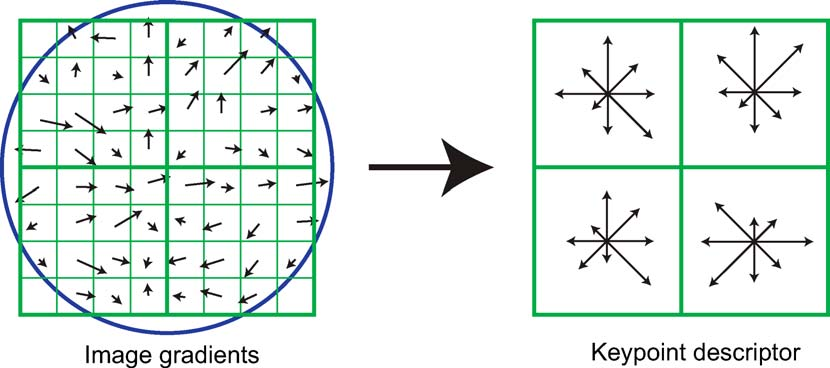
\includegraphics[width=0.8\textwidth]{Figures/sift/descriptor.jpg}
    \caption[Extracting the sift-descriptor.]{Building of the sift-descriptor. \cite{Lowe2004}}
    \label{fig:sift_descriptor}
\end{figure}
